\subsection{Layer Summarization}
\label{sec:exp_layer_summaries}

In this set of experiments we hope to show that we can recover introduced perturbations of input images by examining layer summaries. We hope to see that when classification changes occur, perturbations cause changes through in the summaries of all layers. Whereas when a perturbation does not cause a classification change, a perturbation should become less noticeable in the deeper layers of the network.

We now evaluate qualitatively layer summarization on perturbed images. At a high level, we found that layer summarization is most helpful in validating observations found by our clustering technique. We do this by introducing specialized perturbations to the image, including changing the image hue or removing whole objects with photo manipulation tools. We then compare the summaries for the original image and the perturbed image. the images in all are min-max normalized to best visualize their contents.

Based on our observations from clustering we introduce two kinds of errors to our example images. Namely modifying the hue slightly, as to not change the semantic meaning of the image, and removing whole objects from the image. While we initially attempted to remove objects by replacing them with black regions, we found that this technique added undesirable information, namely large black regions and color to black transitions in the images that may adversely impact classification performance. We eventually decided on manipulating the images by replacing objects patches cloned from nearby areas using a photo manipulation tool. Example of this manipulation is found in the second rows of both both Figure \ref{fig:living_room_ls_fig} and Figure \ref{fig:aquarium_ls_fig}. 

\begin{figure}[tbp]
\centering
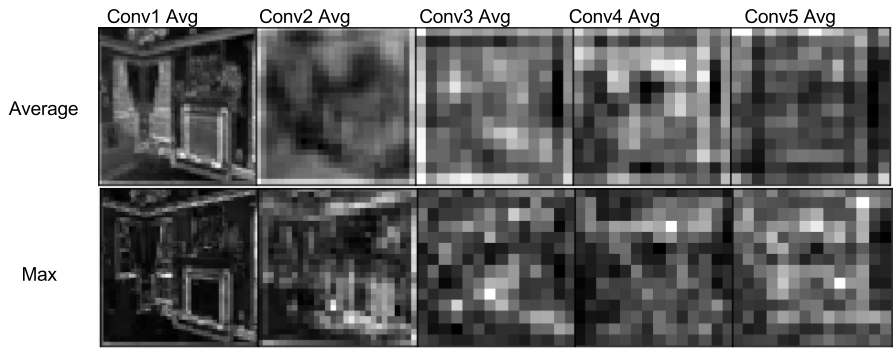
\includegraphics[width=\columnwidth]{figures/layer_summary/avg_vs_max_layer_summary}
\caption{Comparison of Maximum and Average Layer Summary}

\label{fig:avg_vs_max_fig}
\end{figure}

The choice of the aggregation function has a direct impact on the quality and type of information available in a layer summary. We explored two aggregation functions for layer summaries: average and maximum. While the average summary contains contributions from every unit in a layer equally, it is possible that we will not be able to detect large changes in a small number of layers. Alternatively aggregating using a max may miss changes in a large number of layers. In Figure \ref{fig:avg_vs_max_fig} we compare the maximum and average summaries for an example living room image. We found that in both this example and for most of our test images, that the average summary was more useful in finding trends in the summary differences. The maximum images were too noisy to gain meaningful insight into the behavior of the network. There are a wide range of other possible aggregation techniques, including taking the top n\% of activated pixels or a more intelligent scheme based on the weights of the network. We leave this as future work.

\begin{figure}[tbp]
\centering
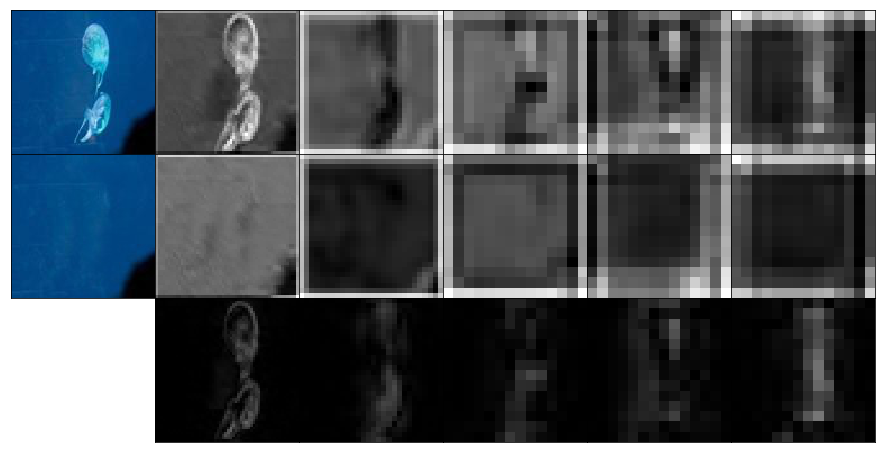
\includegraphics[width=\columnwidth]{figures/layer_summary/aquarium_diff_fig}
\caption{Difference of Layer Summaries in a manipulated image}

\label{fig:aquarium_diff_fig}
\end{figure}

We evaluate the quality of layer summaries by visually comparing the changes in intermediate layers observed by adding perturbations to our images. Comparing the layer-by-layer summaries of an original and a perturbed image reveals changes in the aggregate activations in a layer that may lead to change in the prediction of the network. The process of generating summaries and comparing them for an original image and a perturbed image is demonstrated in figure ~\ref{fig:layer_summary_fig}. Figure ~\ref{fig:aquarium_diff_fig} shows an example of this difference. The top row contains the original image followed by a layer summary of each convolutional layer in our Alexnet model from \texttt{conv1}  to \texttt{conv5}. The second row contains the manipulated image with the fish removed, and its layer summaries. The last row contains the pixel-wise difference of the summaries from the original and manipulated image. While we observe that our manipulation still produces visible effects in the later layers of the network, we reason that the changes in inner pixels were not ultimately important for the classification as the modified image is still classified as an aquarium. 

\begin{figure}[tbp]
\centering
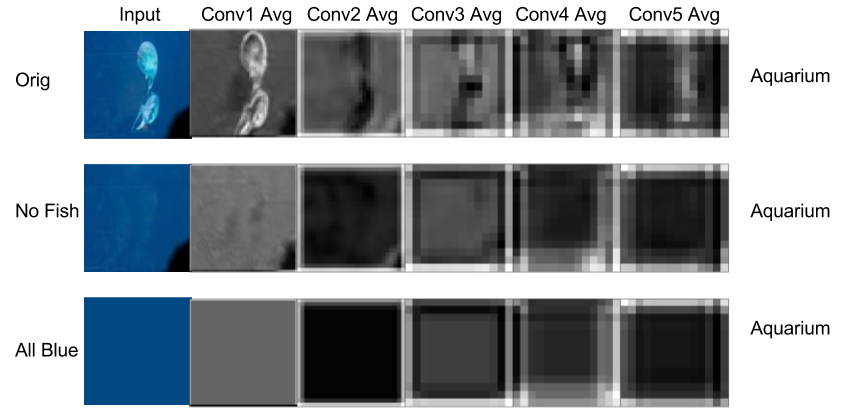
\includegraphics[width=\columnwidth]{figures/layer_summary/aquarium_fig}
\caption{Comparison of Perturbed Aquarium Image with Classification from Alexnet model}

\label{fig:aquarium_ls_fig}
\end{figure}

\begin{figure}[tbp]
\centering
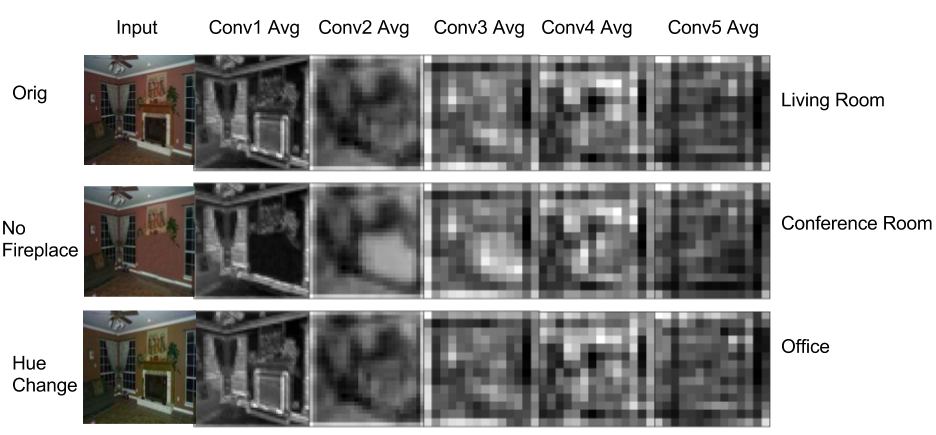
\includegraphics[width=\columnwidth]{figures/layer_summary/living_room_fig}
\caption{Comparison of Perturbed Living Room Image with Classification from Alexnet model}

\label{fig:living_room_ls_fig}
\end{figure}

As the removal of the only recognizable object in the aquarium image did not change the classification result of our network, we deduced that color was one of the most important features for the 'aquarium' class. To further validate this result, we created an artificial image where every pixel is set to the average blue found in the source image. As seen in Figure \ref{fig:aquarium_ls_fig}, none of these changes led to a change in our networks classification, even when all semantic information except color was removed.

We performed similar manipulations on a correctly classified living room image to validate results from clustering indicating depended on detecting objects including furniture in the images. Figure \ref{fig:living_room_ls_fig} shows the original and manipulated images with their respective average layer summary, and the final prediction of our Alexnet model. The first manipulation removes the fireplace, and the second manipulation tweaks the hue of the input image. By comparing the layer summaries for original image and the image without a fireplace, we see that this change has a strong impact on many layers of the network even through \texttt{conv5}. The effect is strongest in the area where the fireplace is removed, and may explain the misclassification. In this case the correct prediction dropped from the networks first rank to it's seventh rank. The second manipulation was a hue change, we found changes of this type much more difficult to detect in layer summary images compared to removing whole objects. 

These experiments may suggest data augmentations that can be added during training to better cover the sets of example on which a given model performs poorly. For instance, we find that some classes are more sensitive to manipulations than others. Some ``aquarium'' images could have nearly all of their semantic content removed while still remaining correctly classified, while some ``living room'' images were more sensitive to these changes. These summarizations were only able to detect some types of perturbations. 